\section{Introduction}

\subsection{Balanced \textit{k}-Mean}
	\begin{frame}{Balanced \textit{k}-Means} % FIXME: reorder 3 elements`
		\small
		\begin{minipage}{0.45\textwidth} % FIXME: padding
			\textbf{Outline}
			\begin{itemize}
				\item[$\bullet$] QUBO formulation and theoretical analysis
				\item[$\bullet$] Empirical Analysis 
				\item[$\bullet$] Authors' Conclusions
				\item[$\bullet$] Our Conclusions, opinions and considerations
			\end{itemize}
			\textbf{Advantages over classical approaches}
			\begin{itemize}
				\item[$\bullet$] Better targets the global solution of the training problem  
				\item[$\bullet$] Better theoretic scalability on large datasets
			\end{itemize}
		\end{minipage}\hfill
		\begin{minipage}{0.55\textwidth}
			\hspace{0.2cm}
			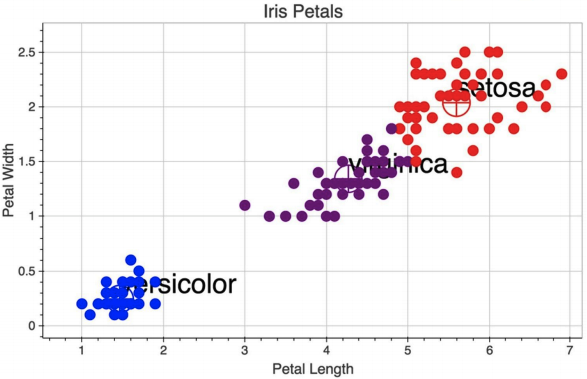
\includegraphics[scale=0.3]{Iris.png}
		\end{minipage}
	\end{frame}
	% NOTES2: The paper we are going to talk about proposes a quantum implementation of Balanced k-Means, which is a clustering algorithm that aims at clustering data in similar sets which have the same number of samples inside them. 
	% The similarity is measured by statistical variance within each cluster

	% You can see here the outline of our presentation...
	
	% why should we look for a Q-algorithm for this problem?

	% The advantages over classical approaches are…


\subsection{Unconstrained \textit{k}-Mean Clustering}
	\begin{frame}{Unconstrained \textit{k}-Mean Clustering}
		\textbf{Lloyd’s algorithm}
		\begin{itemize}
			\item[$\bullet$] Complexity $O(Nkdi)$ \textcolor{gray}{[13]}
			\begin{itemize}
				\item[$\circ$] $N$ number of data points
				\item[$\circ$] $k$ number of clusters 
				\item[$\circ$] $d$ number of features
				\item[$\circ$] $i$ number of iterations before the algorithm converges
			\end{itemize} 
		\end{itemize}
		\textbf{Scikit-learn implementation}
		\begin{itemize}
			\item[$\bullet$] Complexity $O(Nkd)$ \textcolor{gray}{[18]}
		\end{itemize}
		\bigbreak
		\tiny{ % FIXME: attach to bottom
			\textcolor{gray}{
					[13] J. A. Hartigan and M. A. Wong, “A K-Means clustering algorithm” Applied Statistics 
			}
			\smallbreak
			\textcolor{gray}{
					[18]“Scikit-learn: Machine learning in python,” J. Mach. Learn. Res.
			}
		}
	\end{frame}

	% Throughout the presentation we will compare the quantum representation
	% to other implementation of the same problem or its "unconstrained" (not
	% balanced) counterpart. 
	
	% Lloyd’s algorithm is an iterative approach for solving unconstrained 
	% k-means clustering (meaning that the result is not necessarily balanced). 
	% The complexity is….

	% The authors use the Scikit-learn implementation (which bounds the number of iterations) as a point of comparison.

\subsection{Balanced \textit{k}-means clustering}
	\begin{frame}{Balanced \textit{k}-means clustering}
		\textbf{Malinen et al.}
		\begin{itemize}
			\item[$\bullet$] Complexity $O(N^3)$ \textcolor{gray}{[13]}
		\end{itemize}
		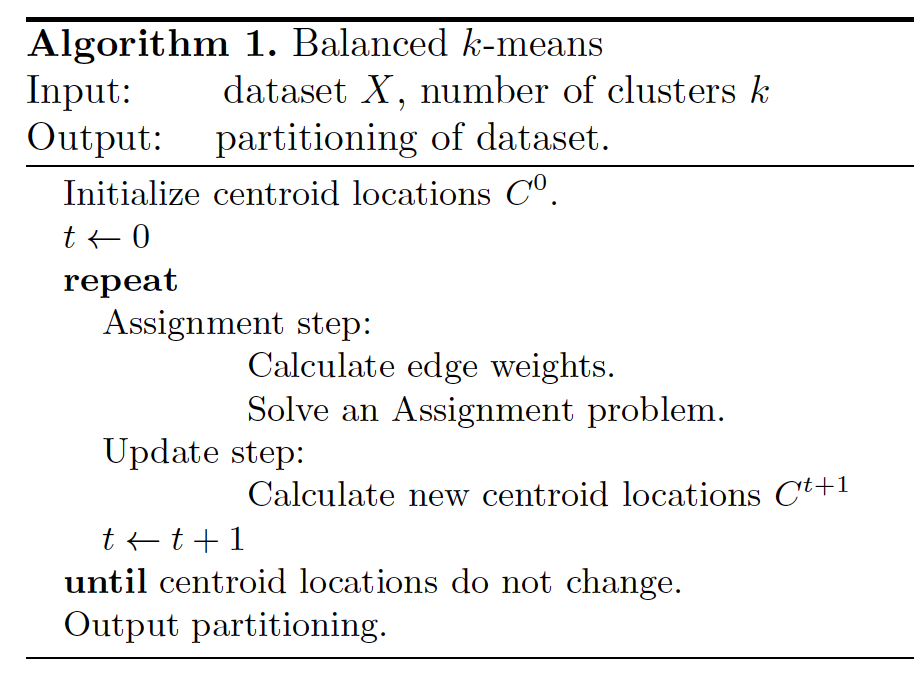
\includegraphics[width=6cm]{[21]algorithm.png}
		\break
		\tiny{ % FIXME: attach to bottom and add margin
			\textcolor{gray}{
				[21] Malinen, Mikko. (2014). Balanced K-Means for Clustering. 
			}
		}
	\end{frame}

	% this is the other algorithm is used for comparison. It is a balanced,
	% k-means algorithm and it has complexity O(N^3)

\subsection{QUBO formulation}
	\begin{frame}{QUBO formulation}
		\begin{columns}
			\begin{column}{0.5\textwidth}
				% 1 
				$$\min _{z \in \mathbb{B}^{M}} z^{T} A z$$
				\pause
				% 2
				$$X=\left\{x_{1}, x_{2}, \ldots, x_{N}\right\}$$\\$$\Phi=\left\{\phi_{1}, \phi_{2}, \ldots, \phi_{k}\right\}$$
				\pause
				% 3 
				$$\min _{\Phi} \sum_{j=1}^{k} \sum_{x \in \phi_{j}}\left\|x-\mu_{j}\right\|^{2}$$
				\pause
				% 4
				$$\min _{\Phi} \sum_{j=1}^{k} \frac{1}{2\left|\phi_{j}\right|} \sum_{x, y \in \phi_{j}}\|x-y\|^{2}$$
				\pause

			\end{column}
			\begin{column}{0.5\textwidth}  
				% 5
				$$\min _{\Phi} \sum_{j=1}^{k} \sum_{x, y \in \phi_{j}}\|x-y\|^{2}$$
				\pause
				% 6
				Distance matrix: $D$ \\Assignment matrix: $\hat W$
				\pause
				% 7
				$$\sum_{x, y \in \phi_{j}}\|x-y\|^{2}=\hat{w}^{\prime \: T}_{j} D \hat{w}_{j}^{\prime}$$
				\pause
				% 8
				$$\min _{\hat{w}} \hat{w}^{T}\left(I_{k} \otimes D\right) \hat{w}$$
			\end{column}
		\end{columns}
	\end{frame}
	% Quantum clustering algorithms have been proposed but the author proposes a QUBO formulation that is identical to the balanced k-means training problem.
	% Our goal is to convert the balanced k-means training problem into a QUBO formulation. 
	% 1-> A is the real valued MxM QUBO matrix while z is the binary decision vector
	% 2-> we want to partition a dataset of N samples into k clusters
	% 3-> This is the original problem, mu is the centroid of a cluster
	% 4-> utilizing the law of total variance
	% 5-> in case we assume the clusters to be balanced we can drop the constant 1/2|\phi|
	% 6-> D: NxN matrix with distances, 
	% 	  W: Nxk matrix with binary values with ones if a sample is assigned to that column's cluster
	% 7-> w_j is the j-th column of W. The first multiplication makes us obtain a n-row vector in which each value is the sum of the distances of 1 of n samples from the samples in the cluster, the second one only select the sum of distances of samples in the same cluster.
	% 8-> \hat w is the vertical stack of column of W, now we need to add the constraint over \hat W through penalties 

	\begin{frame}{Penalties}
		\begin{columns}
			\begin{column}{0.5\textwidth}
				% 1 
				$$\alpha\left(\hat{w}_{j}^{\prime T} \hat{w}_{j}^{\prime}-N / k\right)^{2}$$
				\pause
				% 2
				$$\hat{w}_{j}^{\prime T} \alpha F \hat{w}_{j}^{\prime}$$
				% 3
				$$F=1_{N}-\frac{2 N}{k} I_{N}$$
				\pause
				% 4
				$$\min _{\hat{w}} \hat{w}^{T}\left(I_{k} \otimes(D+\alpha F)\right) \hat{w}$$
				\pause
			\end{column}
			\begin{column}{0.5\textwidth}  
				% 5
				$$\beta\left(\hat{w}_{i}^{T} \hat{w}_{i}-1\right)^{2}$$
				\pause
				% 6
				$$\hat{w}_{i}^{T} \beta G \hat{w}_{i}$$
				% 7
				$$G=1_{k}-2 I_{k}$$
				\pause
				% 8
				$$\min_{\hat{w}}\hat{w}^{T} Q^{T}\left(I_{N} \otimes \beta G\right) Q \hat{w}$$
				\pause
			\end{column}
		\end{columns}
		\bigbreak
		$$\min_{\hat{w}} \hat{w}^{T}\left(I_{k} \otimes(D+\alpha F)+Q^{T}\left(I_{N} \otimes \beta G\right) Q\right) \hat{w}$$
	\end{frame}


	%% COL 1 %%
	% Constraint 1) each cluster has to contain approx N/k points
	% 1) This is the simple version of the constraint, the dot product of a column of W will give us the number of points that if equal to N/k will gives the function minimum
	% \alpha is a hyper parameter, we will se later how to tune
	% 2-3) by computing the square and removing the constant term we obtain the equivalent function whose minium is still N/k but is no longer 0
	% 4) and this is the result our previous problem with the first penalization
	
	%%% NOTES %%%
	%% we obtain a vector with the number of 1's in the column minus the same vector w' with -2N/k instead of ones
	%% now we subtract this -2N/k from the number in the column and we only select the points in the column
	
	%% COL 2 %%
	% 5) Then we need to add the constraint so that each points belongs to one and only one cluster.
	% w_i is a row of  W so the first equation is pretty straight forward, clearly minimal when w_i only contains a single 1
	% 6-7) By using the same trick as before we obtain we obtain the following function
	% 8) This time however we have the constraint for each row in stead of for each column so we need to use the matrix Q which linearly transform the vertical stack of column \hat w in a vertical stack of rows

	\begin{frame}{Hyper-parameters tuning}
		$$\min _{\hat{w}} \hat{w}^{T}\left(I_{k} \otimes(D+\alpha F)+Q^{T}\left(I_{N} \otimes \beta G\right) Q\right) \hat{w}$$
		\bigbreak
		\begin{columns}
			\begin{column}{0.5\textwidth}
				$$\alpha=\frac{\max (D)}{2(N / k)-1}$$
			\end{column}
			\begin{column}{0.5\textwidth}  
				$$\beta=\max (D)$$
			\end{column}
		\end{columns}
		
	\end{frame}

	% Hyper-parameters tuning is very important to ensure that the problem is solved finding the a feasible optimum 
	% To do that we need to define α and β so that they are large enough so that they can the constraints aren't violated but small enough so that the constraints importance isn't too high with respect to the main problem of minimizing the clusters variance. 

	% Max D is the maximum distance found in D

	% The idea is that if the clusters are reasonably defined, the maximum element of D is much larger than the average squared distance between two points in a given cluster.
	% This way violating a constraint almost always penalizes the final value more than a poor assignment
	% By dividing α we make the constraint for a balanced solution less important that the one for ensuring a single assignment for each datum.

	% However there are instances in which the constraints are not satisfied and in this cases simple adjustments are made.
	% • A sample assigned to more clusters only retains the assignment to the cluster with the smallest index
	% • A sample assigned to no cluster gets assigned to the first one

	\begin{frame}{Converting equation into a QUBO}
		$$\min _{\hat{w}} \hat{w}^{T}\left(I_{k} \otimes(D+\alpha F)+Q^{T}\left(I_{N} \otimes \beta G\right) Q\right) \hat{w}$$
		\bigbreak
		$$
			\min _{W} \sum_{l=1}^k \sum_{j=1}^N \sum_{i=1}^N \sum_{m=1}^d w_{i l}\left(x_{i m}-x_{j m}\right)^{2} w_{jl}
		$$
		$$
			+\alpha \sum_{l=1}^{k} \sum_{j=1}^{N} \sum_{i=1}^{N} w_{il} f_{ij} w_{j l}+\beta \sum_{l=1}^{N} \sum_{j=1}^{k} \sum_{i=1}^{k} w_{li} g_{i j} w_{lj}
		$$
		\begin{itemize}
			\item[$\bullet$] Complexity $O(N^2 k d)$ 
		\end{itemize}
		\bigbreak
		\begin{columns}
			\begin{column}{0.5\textwidth}
				\textbf{Malinen et al.}
				\begin{itemize}
					\item[$\bullet$] Complexity $O(N^3)$ 
				\end{itemize}
			\end{column}
			\begin{column}{0.5\textwidth}  
				\textbf{Scikit-learn implementation}
				\begin{itemize}
					\item[$\bullet$] Complexity $O(Nkd)$ 
				\end{itemize}
			\end{column}
		\end{columns}

		\bigbreak		
	\end{frame}

	% By rewriting the equation we can see that the worst case complexity for converting the eq. into a QUBO problem is...
	% as a reminder these are the complexity of the algorithms use for comparison

	%% Francesco Actually says this conclusion...
	% Our conclusion based on this complexity and the Empirical analysis we will se later is that before using the quantum algorithm proposed on a large dataset one should assess how important the balanced constraint really is, since the Scikit learn approach remains asymptotically better.

